\documentclass[12pt]{report}
\usepackage{lingmacros}
\usepackage{tree-dvips}
\usepackage{graphicx}
\usepackage{listings}
\graphicspath{ {images/} }

\begin{document}

\section*{Report Labwork X}

\subsection*{I: How you made up the structure}


Explain:
{\small
\enumsentence{Articles,  magazines, and authors need to split to seprate tables, because they have differen attribute. For example: \"article\" have \"content\" attribute or \"authors\" have \"a\_name\". }}

{\small
\enumsentence{To create relation many-many between \"artice\" and \"magazine\" we will create intermediate table name \"maga\_arti\" include \"a\_id\" and \"m\_id\" and page number of article inside that magazine they referent to.}}

{\small
\enumsentence{We can do the same with \"authors\" and \"article\" tables. Then we have \"author\_article\" allow us to create many-many relation between 2 tables.}}


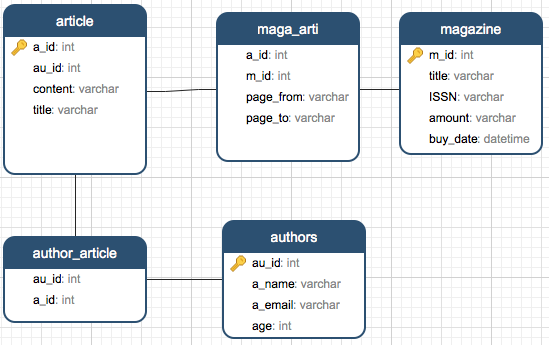
\includegraphics[width=0.7\paperwidth]{labwork10}







\subsection*{II: SQL commands to create the database}

\textbf {Create database}

Create database labwork10 
\begin{lstlisting}[language=sql]

CREATE DATABASE labwork10;

\end{lstlisting}
Output: Query OK, 0 rows affected (0.00 sec)

---------------------------------------------------------------------------------
\\
\textbf {Disable FOREIGN KEY CHECKS}

Disable Foreign key check to create foreign key in tables
 
\begin{lstlisting}[language=sql]

SET FOREIGN_KEY_CHECKS = 0;

\end{lstlisting}
Output: Query OK, 0 rows affected (0.00 sec)

---------------------------------------------------------------------------------\\


\textbf {Table structure for `article`}

Create `article` table with Primary key and two Foreign key 

\begin{lstlisting}[language=sql]
CREATE TABLE `article` (
  `a_id` int(11) NOT NULL AUTO_INCREMENT,
  `au_id` int(11) DEFAULT NULL,
  `content` varchar(255) DEFAULT NULL,
  `title` varchar(255) DEFAULT NULL,
  PRIMARY KEY (`a_id`),
  CONSTRAINT `a_fk` FOREIGN KEY (`a_id`) REFERENCES `author_article` (`a_id`) ON DELETE CASCADE ON UPDATE CASCADE,
  CONSTRAINT `article_fk` FOREIGN KEY (`a_id`) REFERENCES `maga_arti` (`a_id`) ON DELETE CASCADE ON UPDATE CASCADE
);
\end{lstlisting}
Output: Query OK, 0 rows affected (0.01 sec)

---------------------------------------------------------------------------------\\
\textbf {Table structure for `author\_article`}

Create `author\_article` table with two columns

\begin{lstlisting}[language=sql]
CREATE TABLE `author_article` (
  `au_id` int(11) DEFAULT NULL,
  `a_id` int(11) DEFAULT NULL,
  KEY `au_id` (`au_id`),
  KEY `a_id` (`a_id`)
);
\end{lstlisting}

Output: Query OK, 0 rows affected (0.00 sec)

---------------------------------------------------------------------------------\\
\textbf {Table structure for `authors`}

Create `authors` table with Primary key and one Foreign key 

\begin{lstlisting}[language=sql]
CREATE TABLE `authors` (
  `au_id` int(11) NOT NULL AUTO_INCREMENT,
  `a_name` varchar(255) DEFAULT NULL,
  `a_email` varchar(255) DEFAULT NULL,
  `age` int(11) DEFAULT NULL,
  PRIMARY KEY (`au_id`),
  CONSTRAINT `au_fk` FOREIGN KEY (`au_id`) REFERENCES `author_article` (`au_id`) ON DELETE CASCADE ON UPDATE CASCADE
);
\end{lstlisting}

Output: Query OK, 0 rows affected (0.00 sec)

---------------------------------------------------------------------------------
\\
\textbf{Table structure for `maga\_arti`}

Create `maga\_arti` table with two columns

\begin{lstlisting}[language=sql]
CREATE TABLE `maga_arti` (
  `a_id` int(11) DEFAULT NULL,
  `m_id` int(11) DEFAULT NULL,
  `page_from` varchar(255) DEFAULT NULL,
  `page_to` varchar(255) DEFAULT NULL,
  KEY `a_id` (`a_id`),
  KEY `m_id` (`m_id`)
);
\end{lstlisting}

Output: Query OK, 0 rows affected (0.00 sec)

---------------------------------------------------------------------------------
\\
\textbf {Table structure for `magazine`}

Create `magazine` table with Primary key and one Foreign key 

\begin{lstlisting}[language=sql]
CREATE TABLE `magazine` (
  `m_id` int(11) NOT NULL AUTO_INCREMENT,
  `title` varchar(255) DEFAULT NULL,
  `ISSN` varchar(255) DEFAULT NULL,
  `amount` varchar(255) DEFAULT NULL,
  `buy_date` datetime DEFAULT NULL,
  PRIMARY KEY (`m_id`),
  CONSTRAINT `magazine_fk` FOREIGN KEY (`m_id`) REFERENCES `maga_arti` (`m_id`) ON DELETE CASCADE ON UPDATE CASCADE
);
\end{lstlisting}

Output: Query OK, 0 rows affected (0.00 sec)

---------------------------------------------------------------------------------\\
\textbf {Enable FOREIGN KEY CHECKS}

Enable Foreign key check
 
\begin{lstlisting}[language=sql]

SET FOREIGN_KEY_CHECKS = 1;
\end{lstlisting}

Output: Query OK, 0 rows affected (0.00 sec)

---------------------------------------------------------------------------------

\end{document}